\documentclass[12pt]{beamer}

\usetheme{Madrid}
\usepackage{amsmath,amssymb}
\usepackage{graphicx}
\usepackage{tikz}
\usepackage{multicol}
\usepackage{float}

\title{Power Electronics --- Chapter 1}
\subtitle{DC-DC Converters}
\author{POWER\_E\_466}
\date{}



\begin{document}

\frame{\titlepage}

\begin{frame}{Buck Converter:Intro}
	The buck converter is a DC-DC converter that steps down voltage
	($V_{out} < V_{in}$).
	
	\begin{figure}
		\centering
		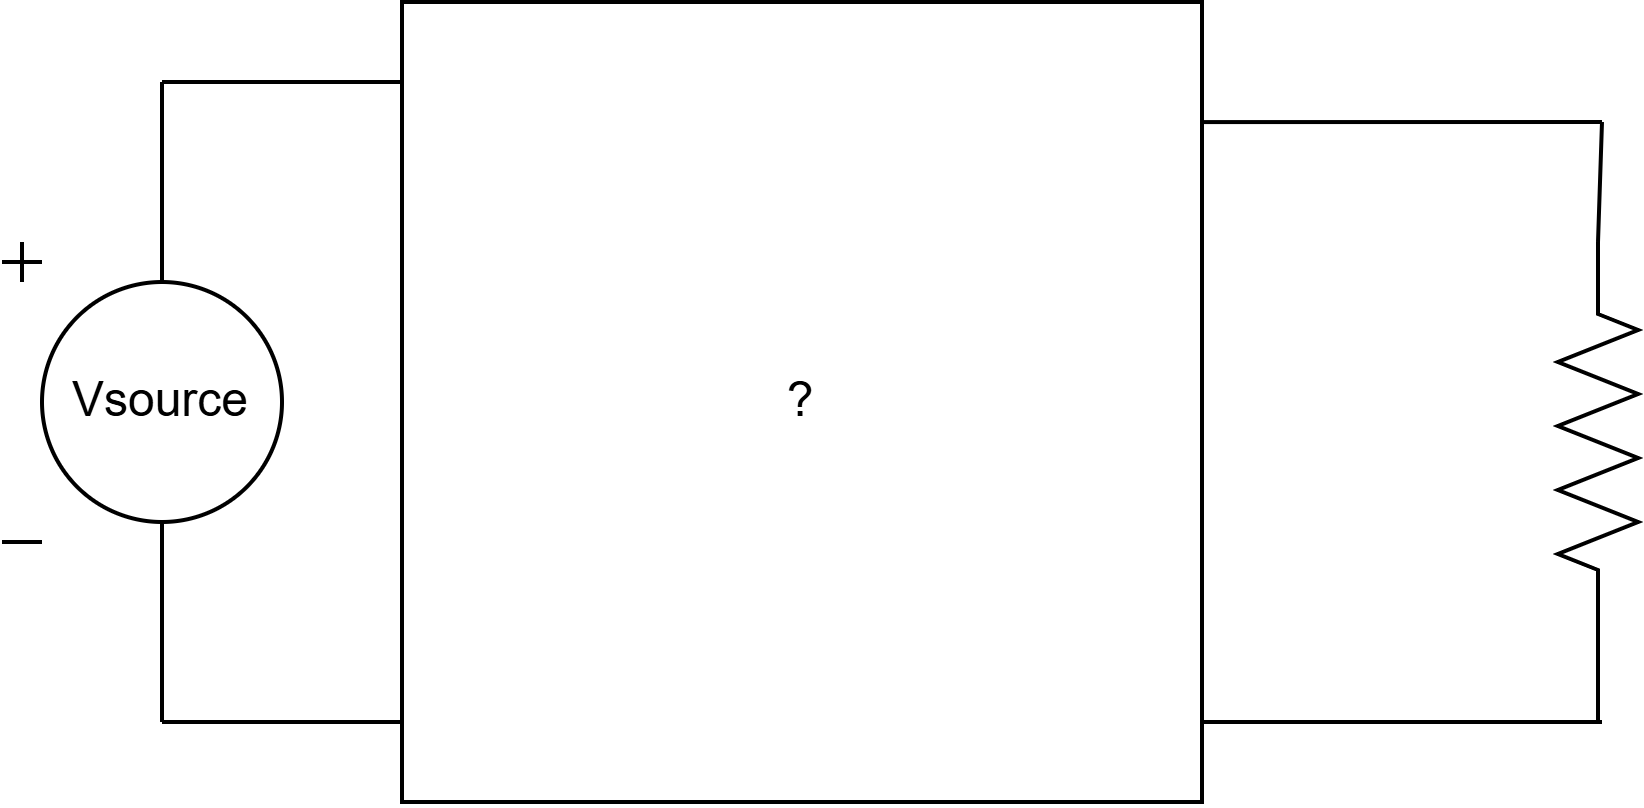
\includegraphics[width=0.7\linewidth]{Graphic/buck_converter/buck_converter_unknow.drawio.png}
		\label{fig:buckconverterunknow}
	\end{figure}
	\vfill
\end{frame}

\begin{frame}{Buck Converter:Switching}
	Start from a black-box model: Given $V_i=50V$, our goal $<V_o>=20v$.\\
	We start with just simple on-off switching.\\
	\begin{figure}
		\centering
		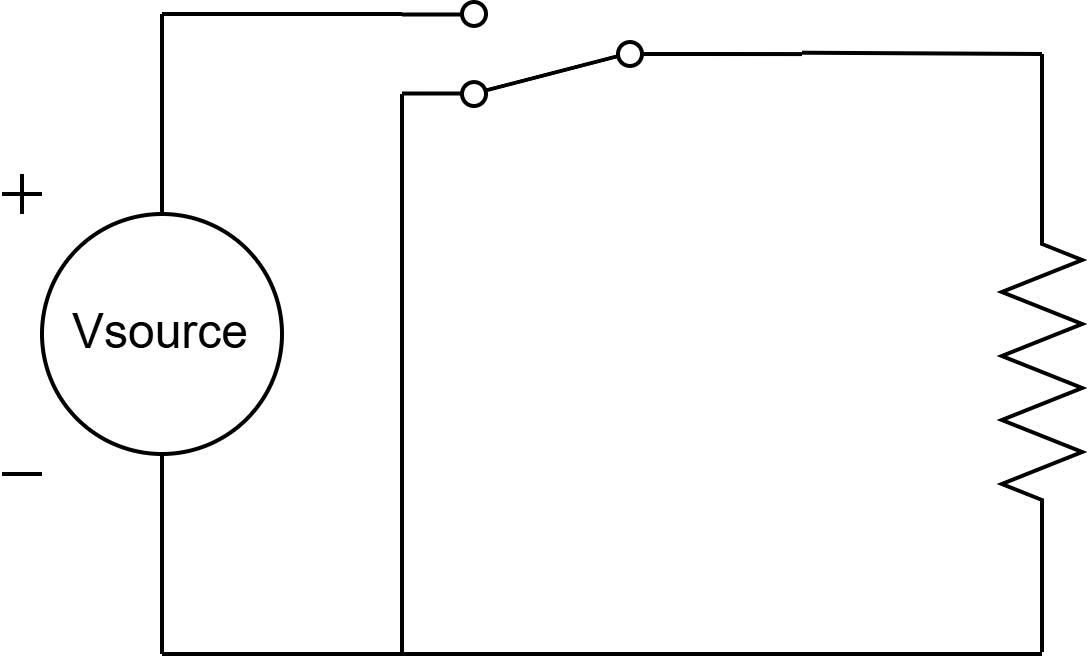
\includegraphics[width=0.7\linewidth]{Graphic/buck_converter/buck_converter_switch_ideal.drawio.png}
		\label{fig:buckconverterswitchideal}
	\end{figure}
	We'll get PWM with average output voltage of 20V
	\vfill
\end{frame}

\begin{frame}{Buck Converter:Filter Added}
	From Fourier we know that DC offset have frequency at 0 hz. $(f=0 \text{ hz})$
	To gain DC offset we used LC filter circuit which lossless in ideal.
	\begin{figure}
		\centering
		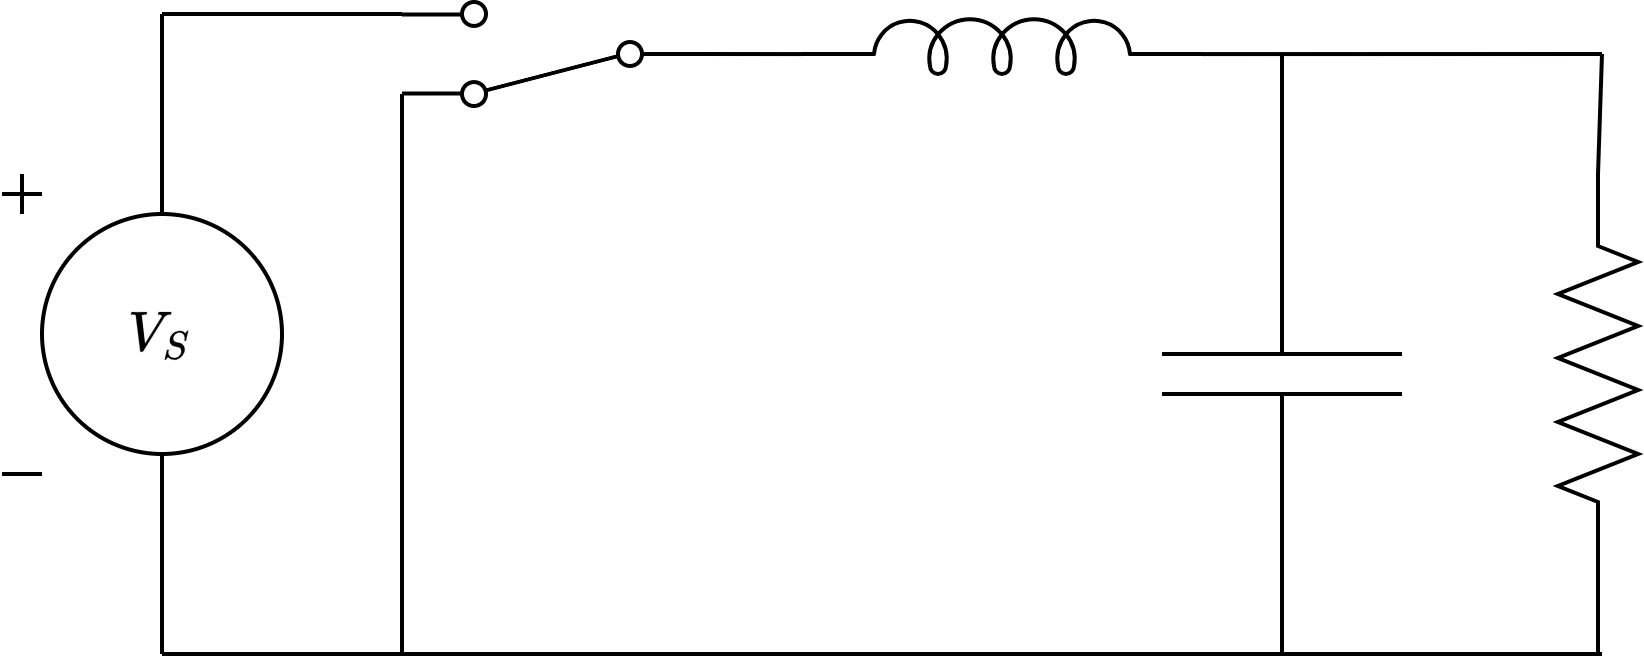
\includegraphics[width=0.7\linewidth]{Graphic/buck_converter/buck_converter_switch.drawio.png}
		\label{fig:buckconverterswitch}
	\end{figure}
	\vfill
\end{frame}

\begin{frame}{Buck Converter:Small Ripple Assumption}
	For an easier circuits analysis we assume the filter provide small  ripple voltage. ($\delta \approx 0$)
	\begin{figure}
		\centering
		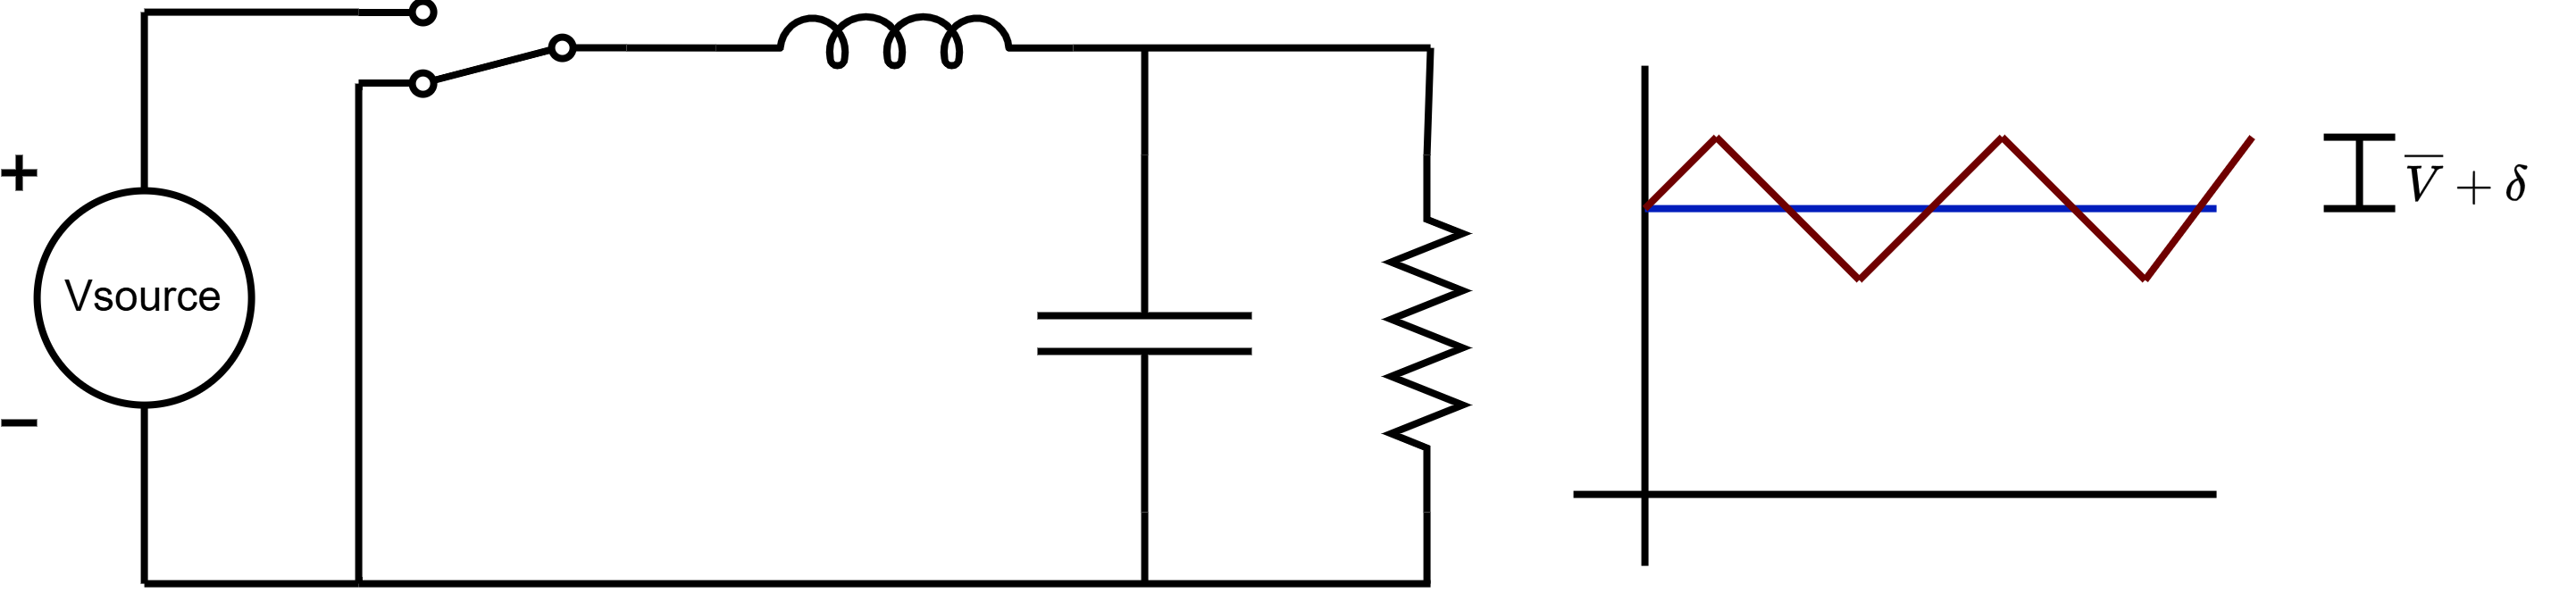
\includegraphics[width=0.9\linewidth]{Graphic/buck_converter/buck_converter_small_ripple.drawio.png}
		\label{fig:buckconvertersmallripple}
	\end{figure}
	We can assume that $V_o$ constant DC offset.
	\vfill
\end{frame}

\begin{frame}{Buck Converter:Inductor and capacitor averaging identities}
	For an inductor,
	\[
	v = L \frac{di}{dt}
	\quad\Longleftrightarrow\quad
	i = \frac{1}{L}\int v \, dt,
	\]
	so if $i$ is periodic in steady state, the average inductor voltage must
	be zero:
	\[
	\langle v_L \rangle = 0 \qquad \text{(volt-second balance)}.
	\]
	
	For a capacitor,
	\[
	i = C \frac{dv}{dt}
	\quad\Longleftrightarrow\quad
	v = \frac{1}{C}\int i \, dt,
	\]
	so if $v$ is periodic in steady state, the average capacitor current
	must be zero:
	\[
	\langle i_C \rangle = 0 \qquad \text{(current-second/charge balance)}.
	\]
\end{frame}

\begin{frame}{Buck Converter:Steady-State Switching On}
	\begin{center}
		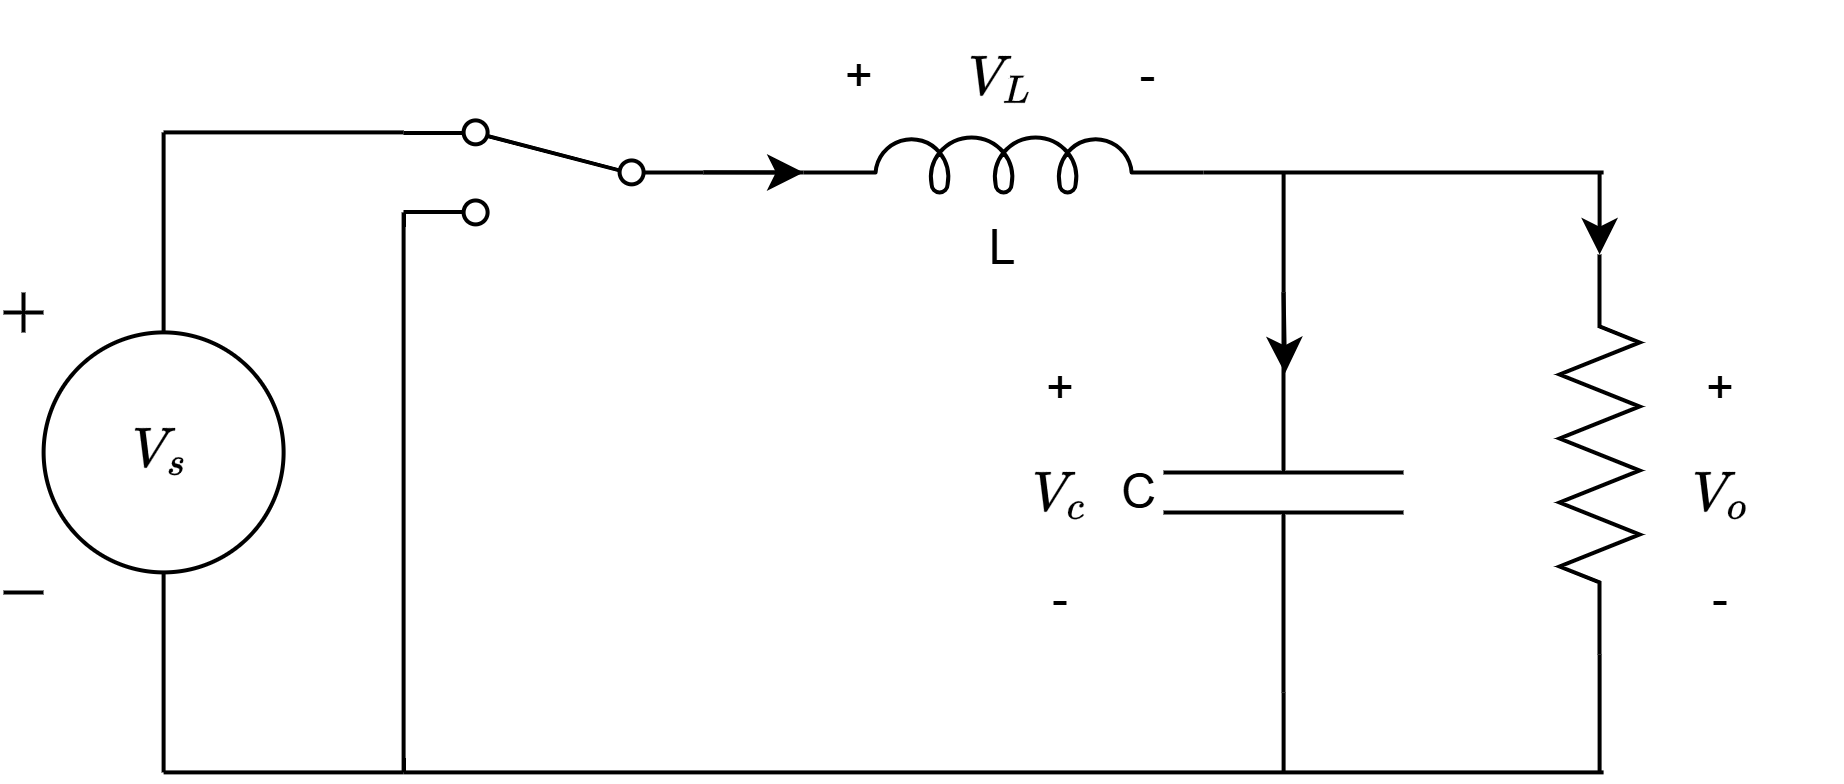
\includegraphics[width=0.7\linewidth]{Graphic/buck_converter/buck_converter_switch_on.drawio.png}
	\end{center}
	\[\frac{di_L}{dt} = \frac{V}{L} = \frac{V_s-V_o}{L}; \space \Delta t = DT; \space \Delta  i_{L \text{-on}} = DT \cdot \frac{V_s-V_o}{L} \]
\end{frame}

\begin{frame}{Buck Converter:Steady-State Switching Off}
	\begin{center}
	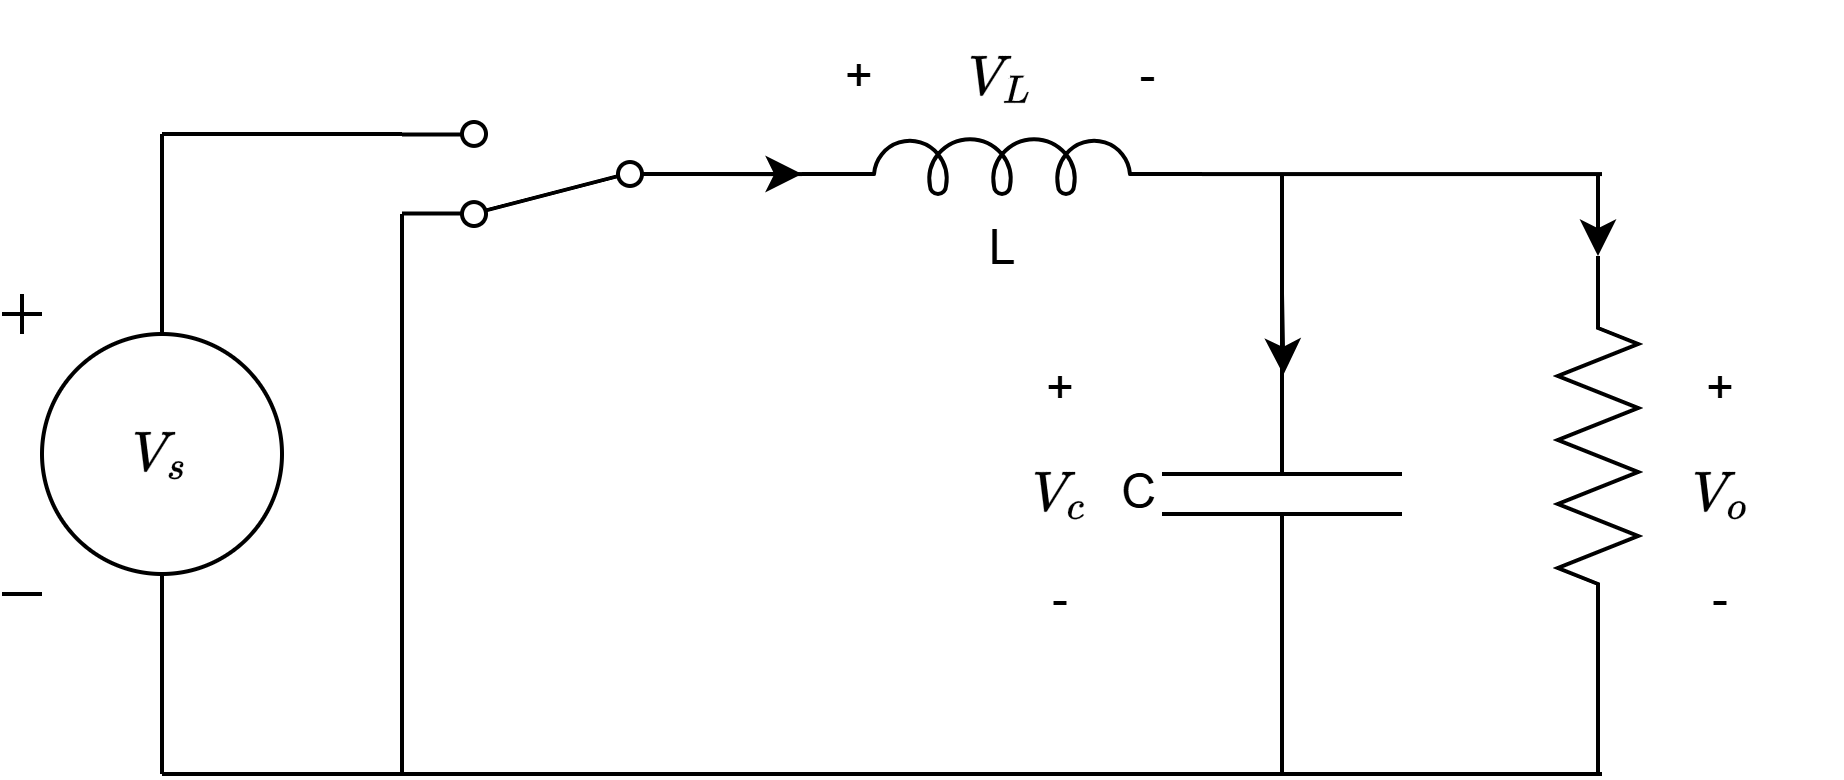
\includegraphics[width=0.7\linewidth]{Graphic/buck_converter/buck_converter_switch_off.drawio.png}
\end{center}
	\[\frac{di_L}{dt} = \frac{V}{L} = \frac{V_o}{L}; \space \Delta t = (1-D)T; \space \Delta i_{L \text{-off}} = (1-D)T \cdot \frac{V_o}{L}  \]
\end{frame}

\begin{frame}{Buck Converter:Steady-State Inductor current}
	\begin{figure}
		\centering
		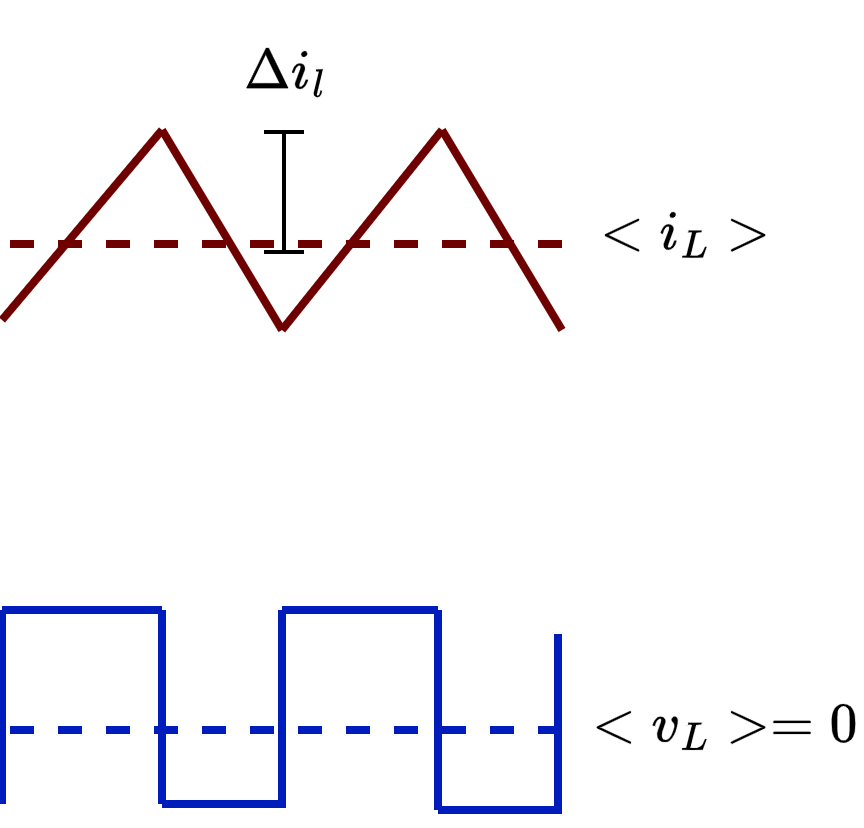
\includegraphics[width=0.4\linewidth]{Graphic/buck_converter/buck_converter_L_VI.drawio.png}
		\label{fig:buckconverterlvi}
	\end{figure}
	
\end{frame}

\begin{frame}{Buck Converter:Transient Switching On (1)}
	For easier analysis we using discrete domain to analyze.
	$V_s=50 \text{V}$ $V_o=0 \text{V}$ $D=0.5$ $L=10 \text{mH}$ $T=1 \text{ms}$ 
	\begin{center}
		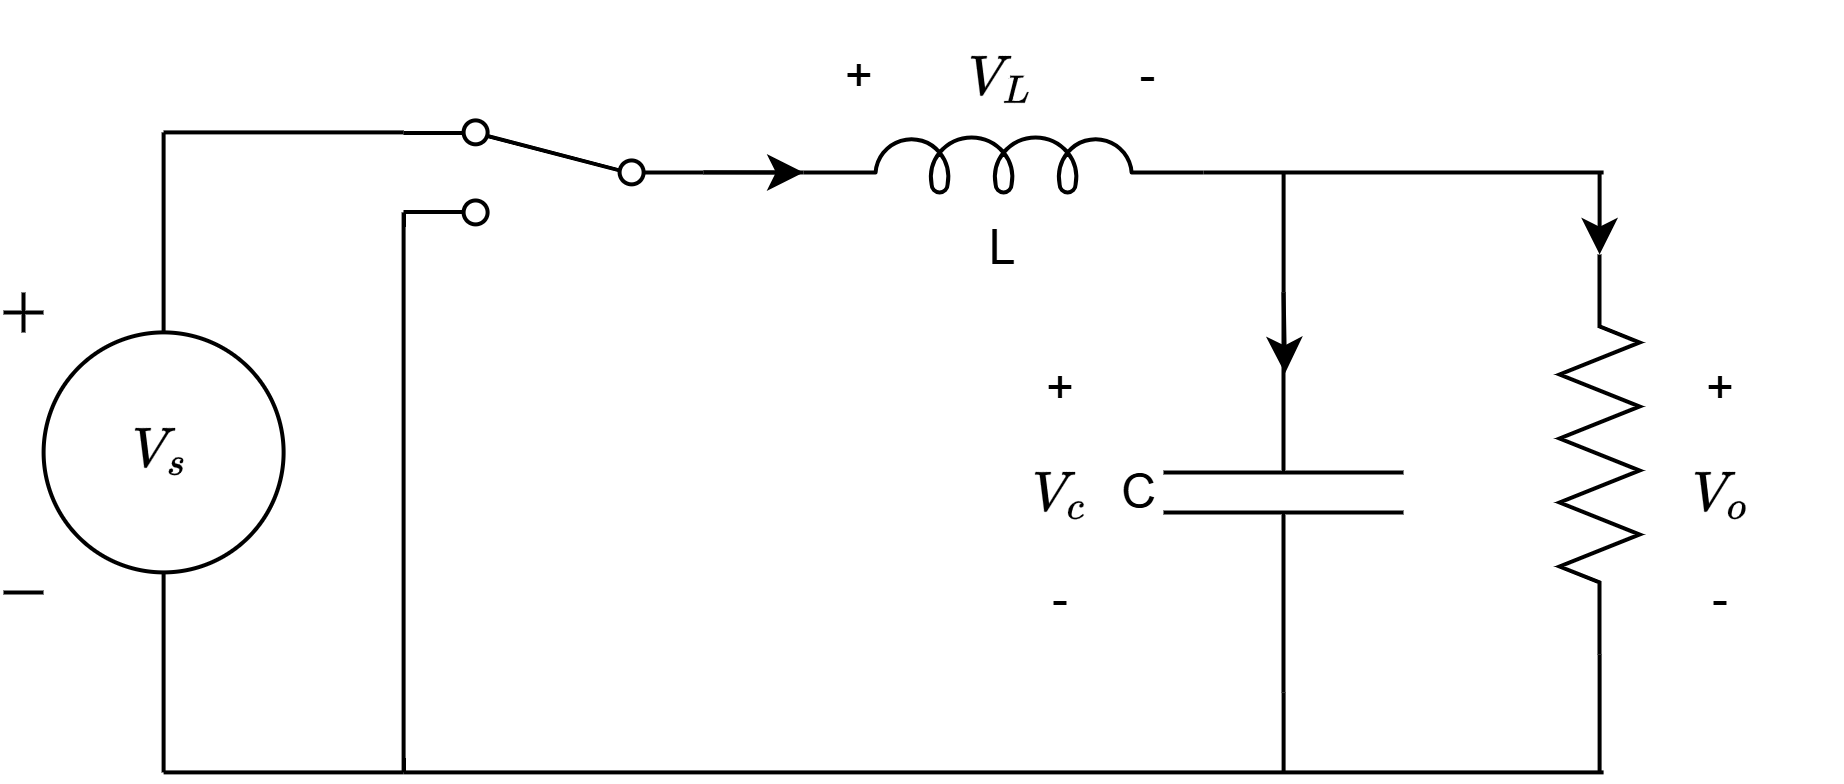
\includegraphics[width=0.7\linewidth]{Graphic/buck_converter/buck_converter_switch_on.drawio.png}
	\end{center}
	\[ \Delta  i_{L \text{-on}} = DT \cdot \frac{V_s-V_o}{L} = 5 \text{A} ; \space i_L = 5 \text{A} \]
	\[ i_c = i_l - i_o = i_l - \frac{V_o}{R} = 5 \text{A} \]
\end{frame}

\begin{frame}{Buck Converter:Transient Switching Off (1)}
	$V_s=50 \text{V}$ $V_o=0 \text{V}$ $D=0.5$ $L=10 \text{mH}$ $T=1 \text{ms}$ 
	\begin{center}
		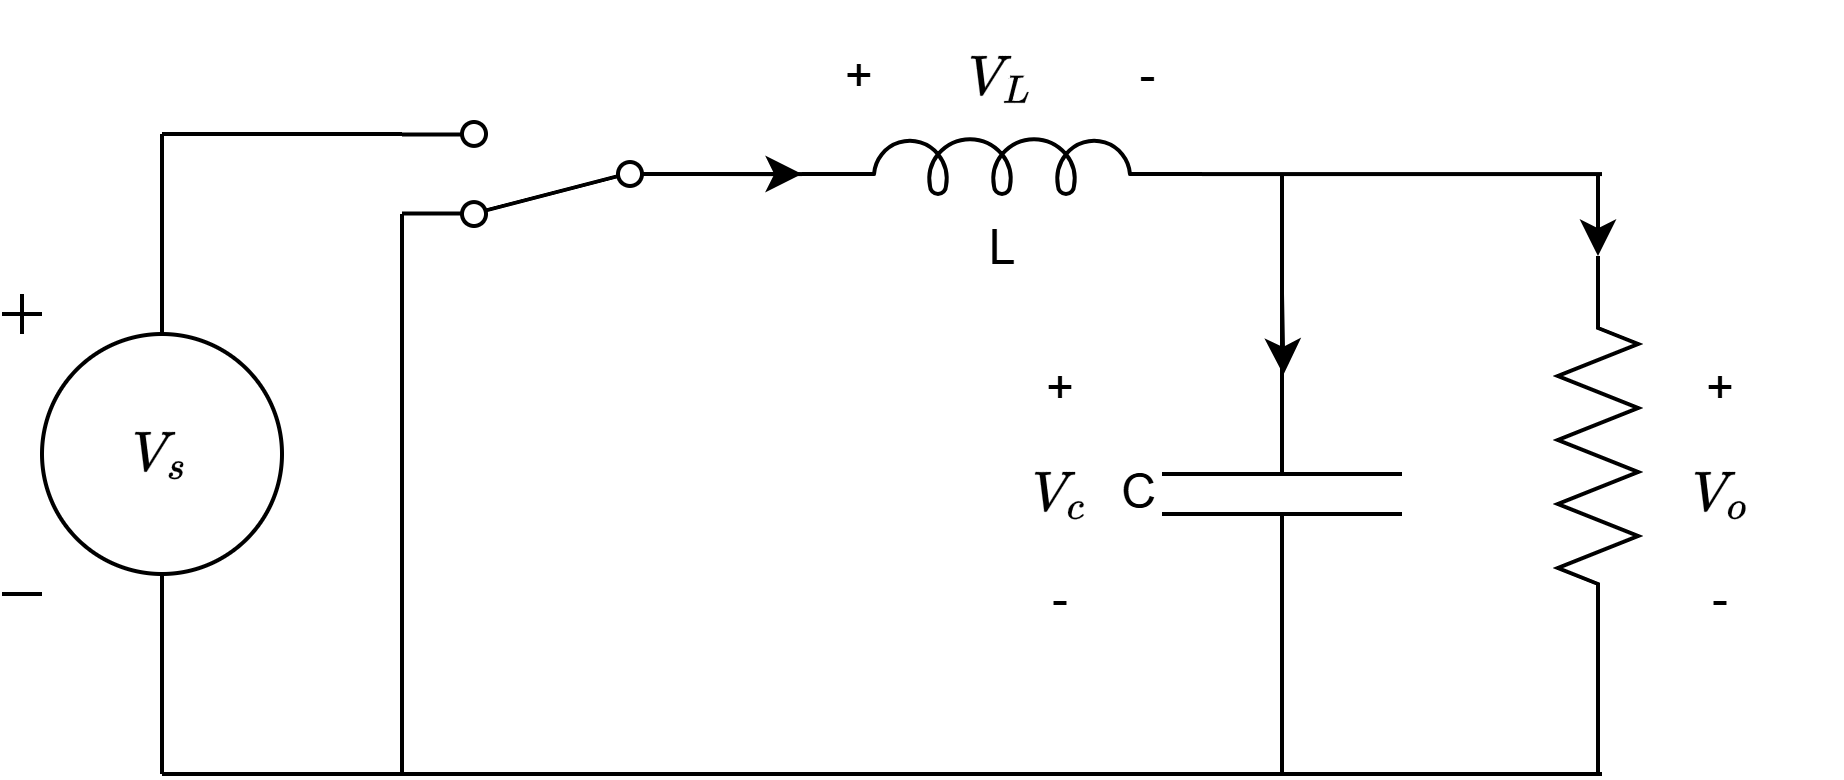
\includegraphics[width=0.7\linewidth]{Graphic/buck_converter/buck_converter_switch_off.drawio.png}
	\end{center}
	\[ \Delta i_{L \text{-off}} = (1-D)T \cdot \frac{V_o}{L} = 0 \text{A} ; \space i_L = 5 \text{A} \]
	\[ i_c = i_l - i_o = i_l - \frac{V_o}{R} = 5 \text{A} \]
\end{frame}

\begin{frame}{Buck Converter:Transient Switching On (2)}
	For easier analysis we using discrete domain to analyze.
	$V_s=50 \text{V}$ $V_o=2.5 \text{V}$ $D=0.5$ $L=10 \text{mH}$ $T=1 \text{ms}$ 
	\begin{center}
		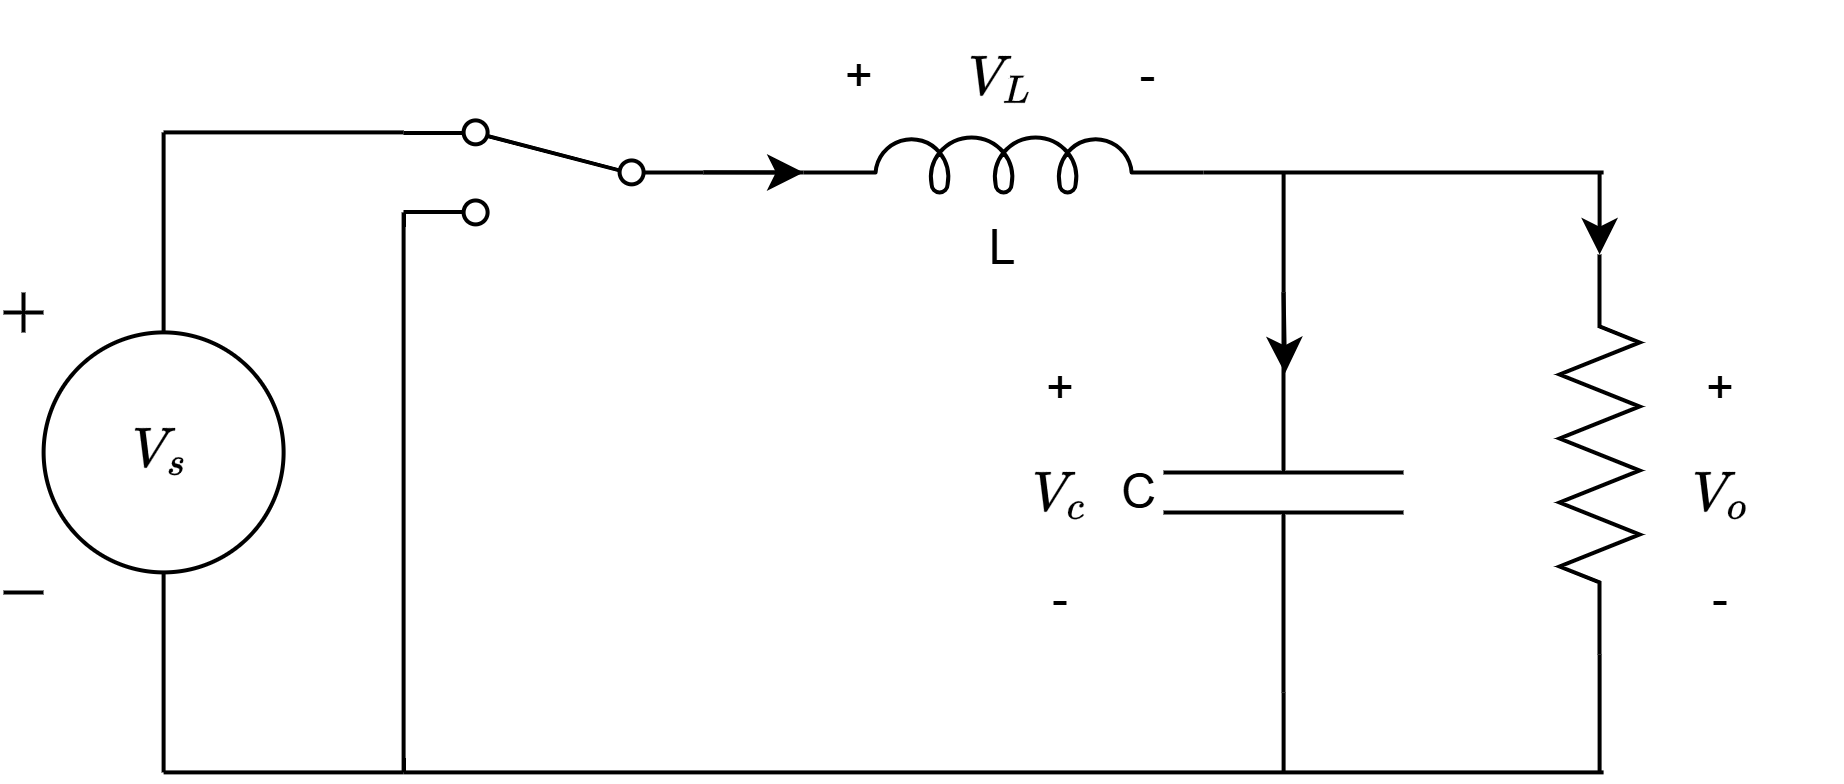
\includegraphics[width=0.7\linewidth]{Graphic/buck_converter/buck_converter_switch_on.drawio.png}
	\end{center}
	\[ \Delta  i_{L \text{-on}} = DT \cdot \frac{V_s-V_o}{L} = 4.75 \text{A} ; \space i_L = 9.75 \text{A} \]
	\[ i_c = i_l - i_o = i_l - \frac{V_o}{R} \]
\end{frame}

\begin{frame}{Buck Converter:Transient Switching Off (2)}
	$V_s=50 \text{V}$ $V_o=2.5 \text{V}$ $D=0.5$ $L=10 \text{mH}$ $T=1 \text{ms}$ 
	\begin{center}
		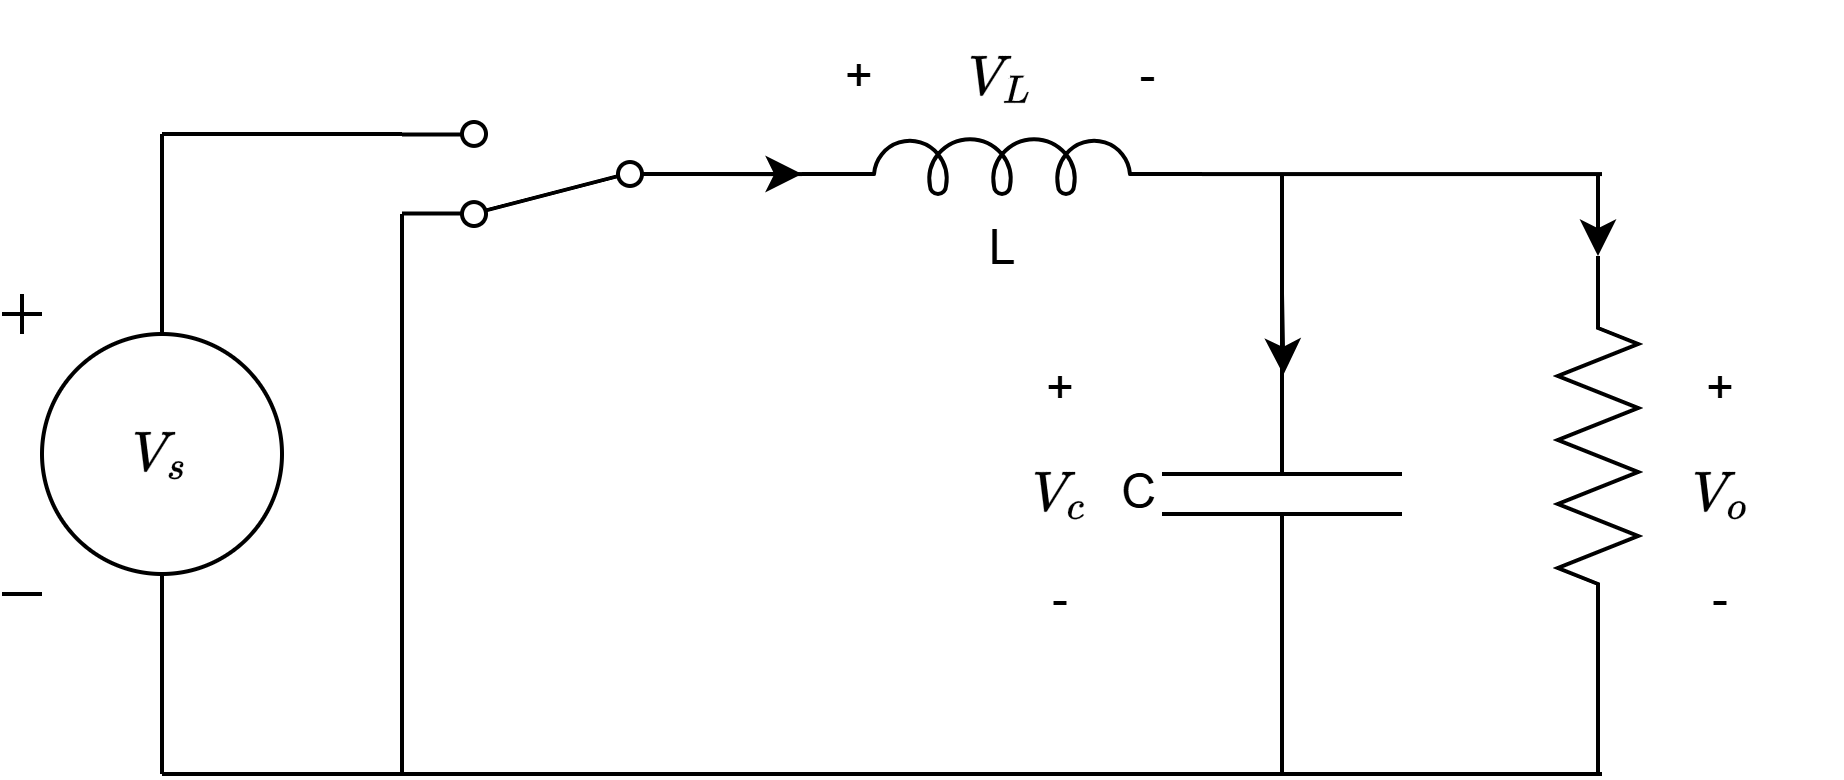
\includegraphics[width=0.7\linewidth]{Graphic/buck_converter/buck_converter_switch_off.drawio.png}
	\end{center}
	\[ \Delta i_{L \text{-off}} = (1-D)T \cdot \frac{V_o}{L} = 0 \text{A} ; \space i_L = 5 \text{A} \]
	\[ i_c = i_l - i_o = i_l - \frac{V_o}{R} \]
\end{frame}

\begin{frame}{Buck Converter:Summary}
	\begin{multicols}{2}
		\begin{figure}[H]
		\centering
			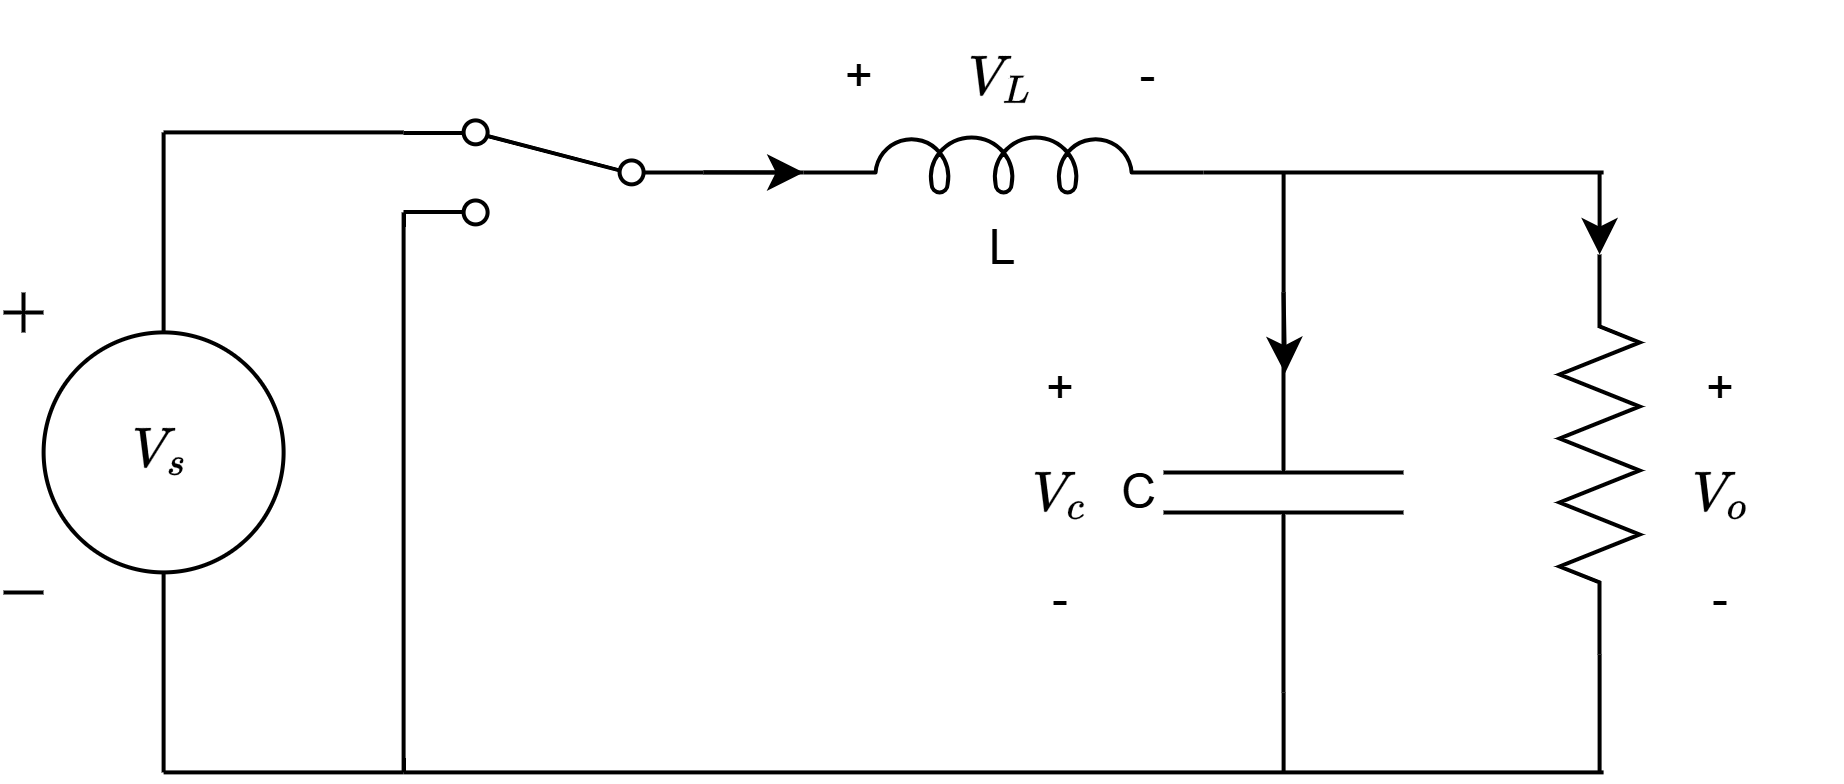
\includegraphics[width=0.8\linewidth]{Graphic/buck_converter/buck_converter_switch_on.drawio.png}
		\end{figure}
		\[\Delta  i_{L \text{-on}} = DT \cdot \frac{V_s-V_o}{L}\]
		\columnbreak
		\begin{figure}[H]
			\centering
			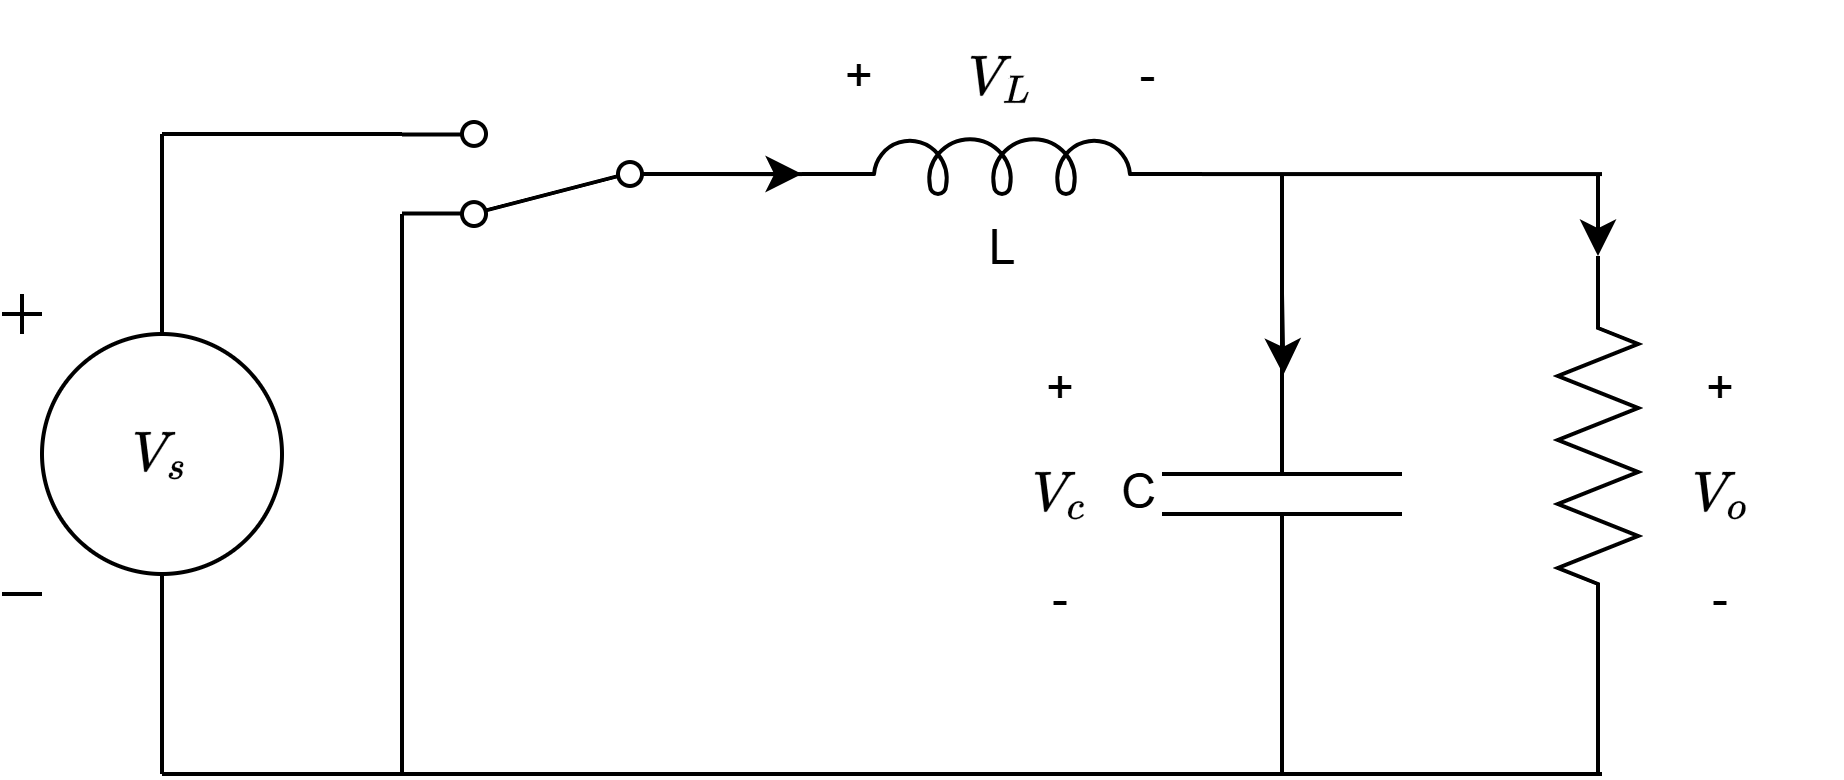
\includegraphics[width=0.8\linewidth]{Graphic/buck_converter/buck_converter_switch_off.drawio.png}
		\end{figure}
		\[ \Delta i_{L \text{-off}} = (1-D)T \cdot \frac{V_o}{L}\]
		\end{multicols}
\end{frame}

\end{document}